\chapter{\textcolor{red}{A non-local $SIR$ model of tree disease (WORK IN PROGRESS)}}

% Introduction...
\blindtext

\blindtext

\subsection{Constructing a generic $SIR$ model} % Describe a Gaussian dispersal model....
\label{section:sgm-expo}
\begin{table}[h]
\centering
\begin{tabular}{l l l}
\hline
\textbf{Model parameter} & \textbf{Description} & \textbf{Typical value(s)}\\
\hline
$\rho$  & Tree density & $0.00 - 0.10$ \\ 
$\beta$ & Infectivity & $0.001 - 0.100\ \mathrm{day}^{-1}$ \\
$\ell$ & Pathogen dispersal distance & $5-30\mathrm{m}$ \\
$T$ & Infectious life-time & $100$ days \\
$t$ & Time-step & $[0, T]$ days\\
$R_0$ & Mean reproduction number & $0-20$ \\
$\mathcal{L}$ & Lattice dimension & $400\times400$ \\
$\gamma$ & Lattice constant & $5\mathrm{m}$ \\
\hline
\end{tabular}
\caption{Model parameters}
\end{table}
% Introduce sub-grid model

%1. Only  scale parameter is present in the dispersal kernel representing short-distance spread. Long distance dispersal effects are not considered.
We begin with a model fixed inside a square lattice of size $\mathcal{L}$ at a resolution of $\mathrm{25m^2}$. At each lattice point a tree is initialised with probability $\rho$, thus generating a random homogeneous distribution of trees over the domain. The probability $\rho$ can therefore be seen as a tree-density parameter. Empty lattice points are insusceptible and denoted by $\emptyset$. The state of a tree can be in one of three conditions: susceptible, infected, or removed\textemdash $SIR$. We assume all trees are equally susceptible and trees that become infected transition through the states $S\rightarrow I\rightarrow R$ without the possibility of recovery.

Given two trees, one susceptible ($S_x$) and one infected ($I_{x^\prime}$), separated by a distance $r=|x - x^\prime|$, an expected transition rate for $S_x \rightarrow I_x$ can be determined from a Gaussian kernel $g(r; \ell)$ multiplied by an infectivity rate $\beta$:
\begin{equation}
    Pr(S_{x} \rightarrow I_{x} ;\ I_{x^{\prime}} ) = \beta \exp\Big[\frac{-r^2}{2\ell^2}\Big]
\end{equation}
where $\ell$ is a distance setting the scale of dispersal. If a tree transitions into the $I$ compartment it will remain infectious for an arbitrary number of $T=100$ days before uniformly transitioning into the $R$ compartment\footnote{Each Monte Carlo step through the simulation is set to be a single day of elapsed time. This is arbitrary (along with $T$) and could be re-scaled.}. A typical simulation through two time-steps is shown in Fig \ref{fig:sgm-evol}(a-b) with parameters $\rho=0.010,\ \ell = 25\mathrm{m},\ \beta=0.05\ \mathrm{day^{-1}}$ on a domain of size $400\times400$ representing an area of $\mathrm{2km^2}$. Model parameters are shown in Table $1$.

\begin{figure}
    \centering
    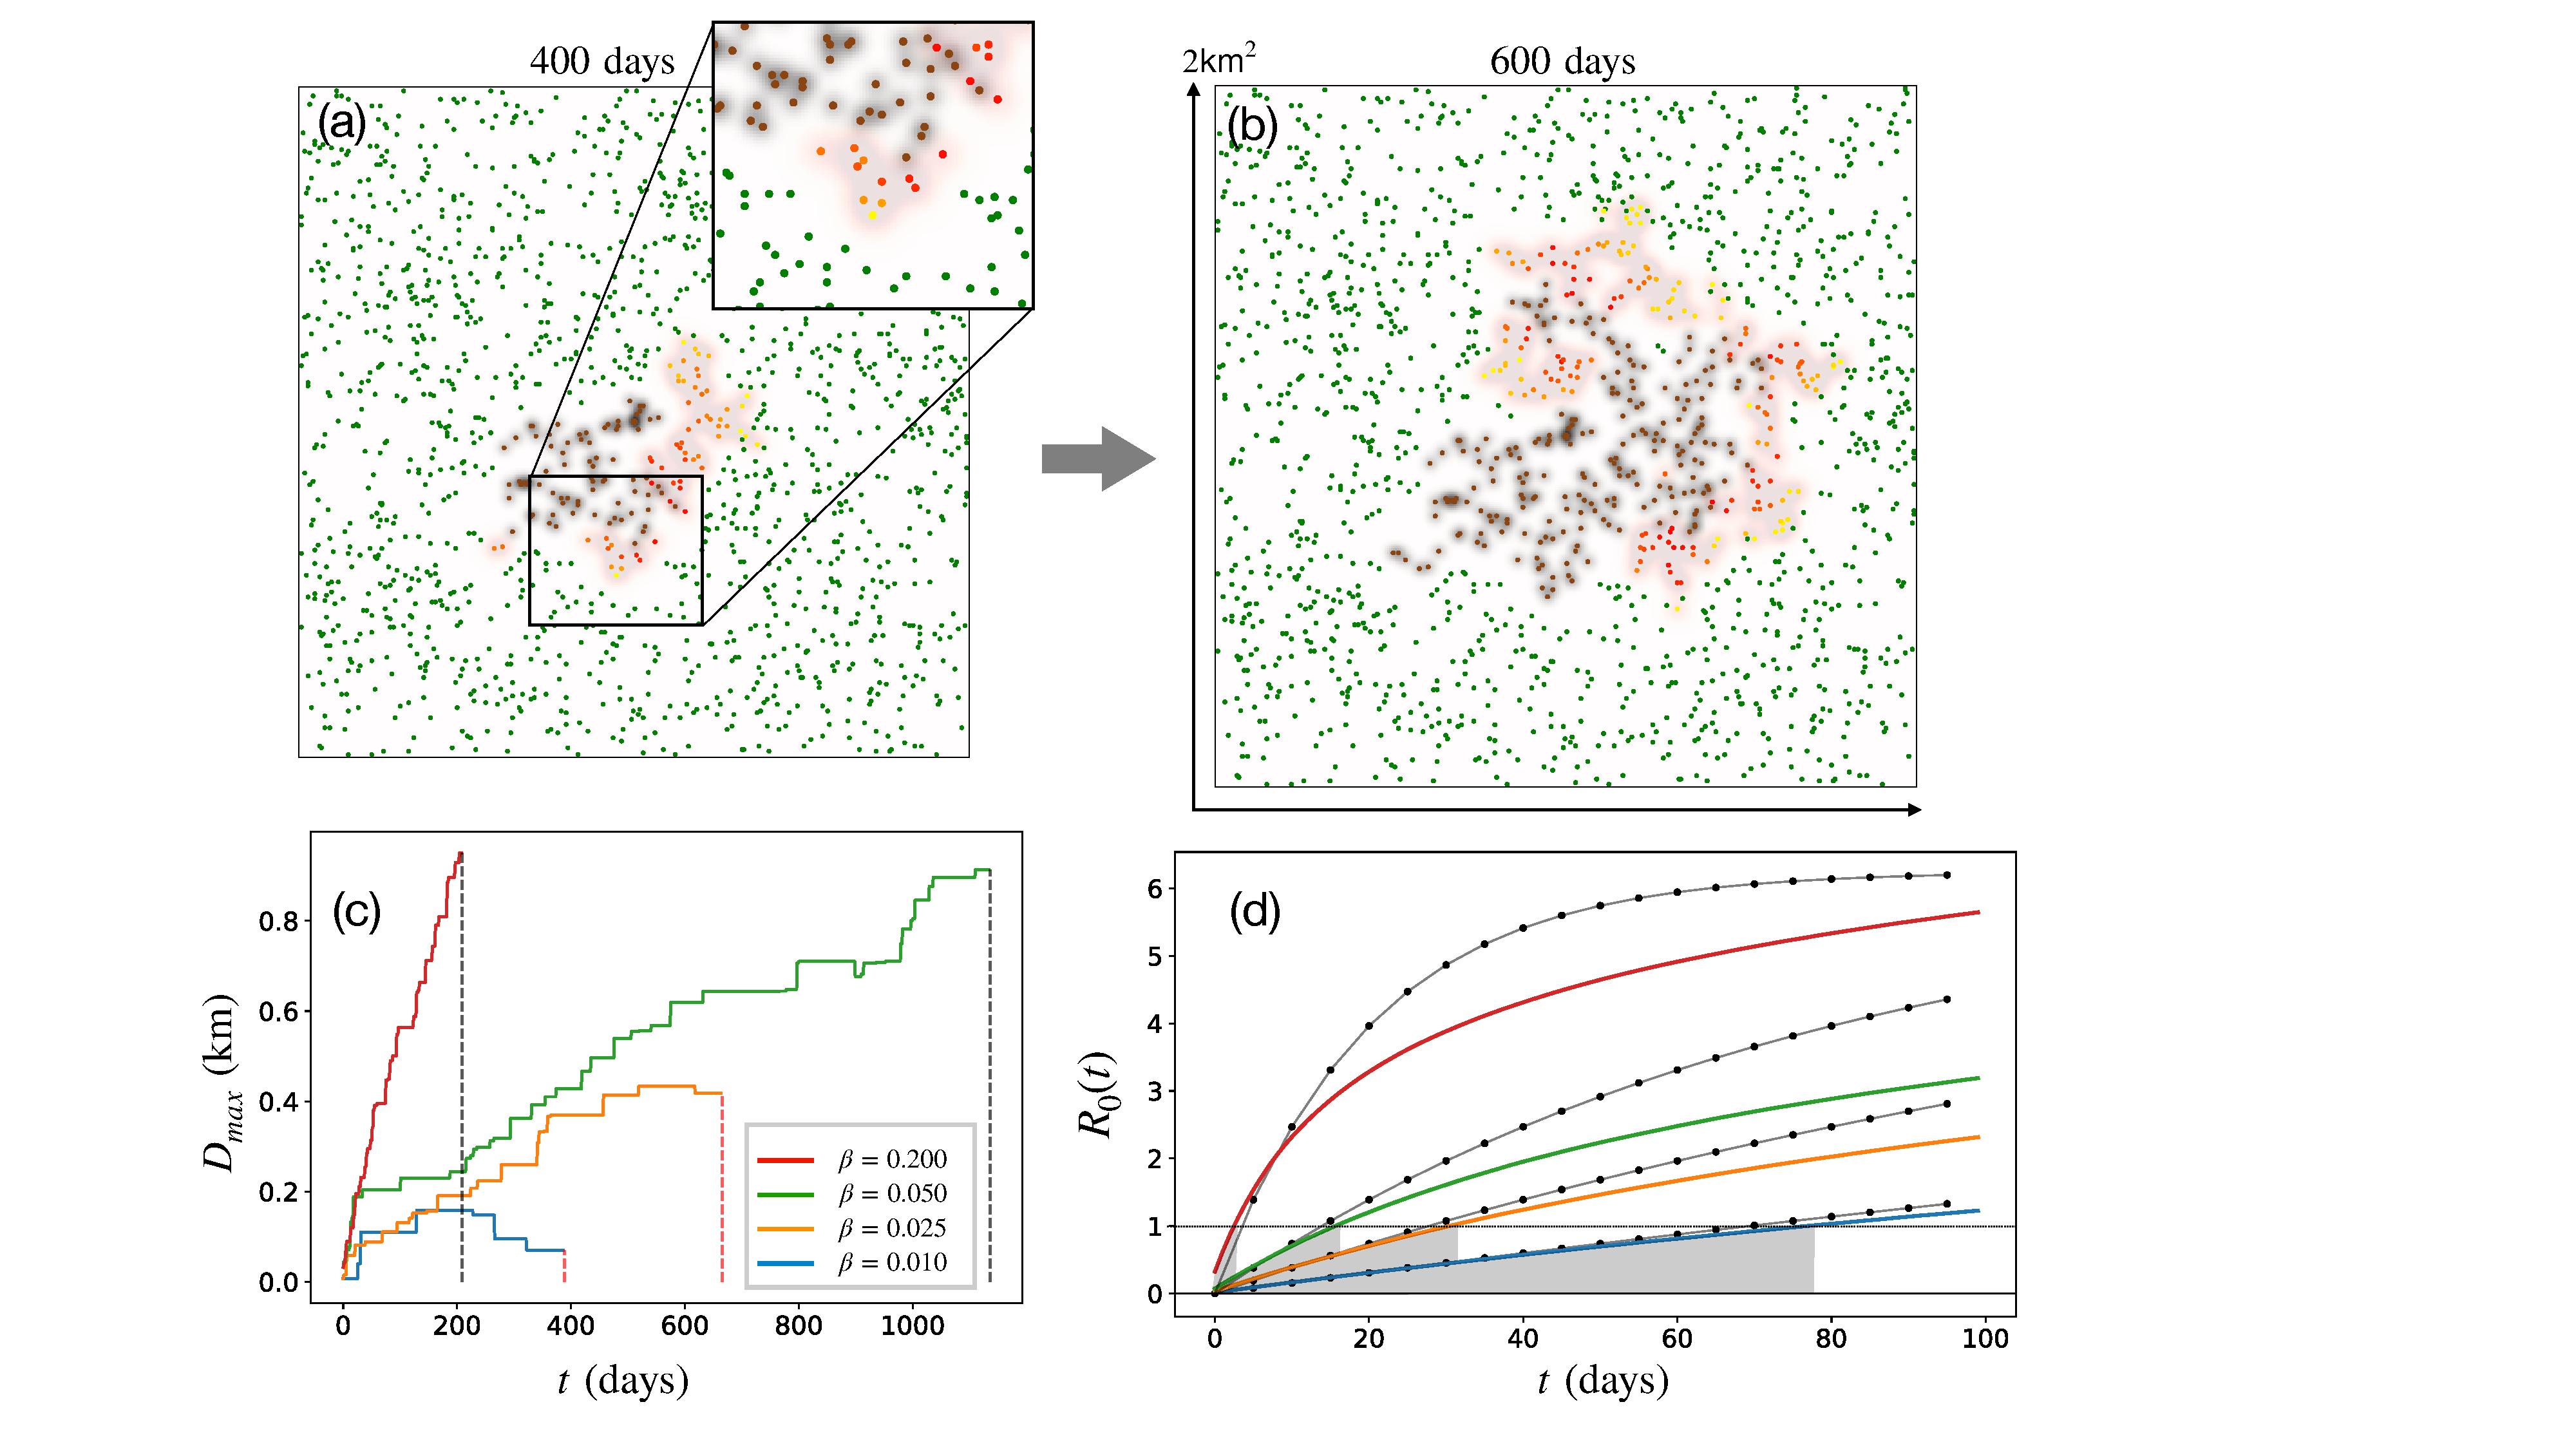
\includegraphics[scale=0.325]{chapter5/figures/figure1.pdf}
    \caption{Stochastic dispersal in the sub-grid model is shown through two time-steps of 400 (a) and 600 (b) days given parameters $\rho=0.01,\ \ell = 25\textrm{m}\ $ and $ \beta=0.05\ \mathrm{day^{-1}}$. Green pixels represent susceptible trees in $S$, while yellow and red pixels represent infected trees at different different steps in the $I$ category. Infected trees uniformly transition into the removed compartment shown in brown-black. (c) The time-series of maximum distance reached by an infected tree is shown for four typical simulations with parameters $\rho=0.01$, $\ell=25\textrm{m}$ and four variations infectivity. Vertical dashed red lines represent time-steps where the pathogen becomes extinct and dies while vertical black lines show when the pathogen survives to reach the domain boundary. (d) The mean number of secondary infections $R_0(t)$ is shown using the same model parameters as Fig \ref{fig:sgm-evol}(c). The black-dotted curves show the corresponding behaviour predicted from equation (\ref{eq:R0-final}).}
\label{fig:sgm-evol}
\end{figure}

After $t$ time-steps, the maximum distance reached by the pathogen is $D_{max}(t)$. This is found to be a useful metric that dynamically captures a pathogen progressing through the domain. Using the same domain conditions as shown in Fig \ref{fig:sgm-evol}(a-b), the time-series of $D_{max}(t)$ are shown in Fig \ref{fig:sgm-evol}(c) for a single simulation run and four variations of $\beta$. The time-series of $D_{max}(t)$ indicate if the pathogen becomes extinct or propagates to the lattice boundary and survives, shown by the vertical red and black dashed lines respectively. Gaussian dispersal does not permit the pathogen to jump large discontinuous distances, therefore, survival to the boundary defines a connected cluster of infectious-removed trees spanning the domain\footnote{This behaviour in Fig \ref{fig:sgm-evol}(a-b) could be considered an approximation to percolation, given the finite size of $\mathcal{L}$.} representing a small-scale epidemic spreading locally.\\

% It makes sense to define a measure for $R_0$ based on the first generation of infections, given that the first generation has, on average, a higher $R_0$. Choosing an $R_0$ in this manner gives us an upper-bound of invasiveness, which for control, is better than an under-estimate:

\section{Non-local $SIR$ behaviour}

\blindtext

\subsection{Small-scale dispersal}

\blindtext % The probability of percolation...

\subsection{Increasing the scale of dispersal}

\blindtext

\blindtext


\section{An analytic approximation to $R_0$}

% Introduce uses and quantities taken from sub-grid --> R_0
An `effective' reproduction number can be defined through the following thought experiment: consider a single (primary) infected tree surrounded by a random homogeneous distribution of susceptible neighbours. Over the course of it's infectious life-time, the primary infection will lead to $R_0$ secondary infections. If secondary infections are not permitted to produce tertiary infections, the neighbourhood around the primary infection remains untouched by other diseased trees and the reproductive potential of the pathogen can be approximated by $R_0$. This can be directly simulated in a straightforward manner through ensemble-averages of the model.\\

\label{section:apendix_A}
We start from three tree categories, $SIR$, and two trees, $S_x\in S$ and $I_{x^\prime}\in I$ separated by a distance $r=\sqrt{|x^2-x^{\prime 2}|}$. The probability of $S_x$ becoming infected on account of $I_{x^\prime}$ is defined by an un-normalised Gaussian kernel $g(r; \ell) = \exp(-\frac{r^2}{2\ell^2})$ and infectivity constant $\beta$. The probability of transition is then:
\begin{equation}
\label{eq:Appendix_pr_trans}
     Pr(S_x\rightarrow I_x;\ I_{x^\prime}) = \beta \exp(-\frac{r^2}{2\ell^2})
\end{equation}
At time $t=0$, the domain is uniform and has density $\rho_0$. Trees transition through states: $S\rightarrow I\rightarrow R$, with $I$ lasting for $T$ time-steps. Integrating this expression over an infinite domain gives $R_0(t=0)$, i.e. the total number of expected infections during the first time-step:
\begin{equation}
    R_0(t = 0) = \beta \rho_0 \int^{\infty}_{-\infty} \exp\Big(-\frac{r^2}{2\ell^2}\Big)dr= 2\pi\beta\rho_0\ell^2
\end{equation}{} 
Assuming no host (re-)growth, at time-step $t+1$ there are less trees to infect. The tree density $\rho$ can therefore be seen as a monotonically decreasing function of time $\rho(t)$, leading to the expression:
\begin{equation}
    R_0(t) = 2\pi\beta\ell^2\rho(t)
    \label{eq:r0-A}
\end{equation}{}
This presents a convenient relationship between tree density and the number of expected secondary infections. In a finite domain of size $\mathcal{L}$ this is given by:
\begin{equation}
    \frac{d\rho}{dt} = - \frac{R_0(t)}{\mathcal{L}^2} = -\frac{2\pi\beta\ell^2\rho(t)}{\mathcal{L}^2}
\end{equation}
Solving the above, with initial condition $\rho_0$ at $t=0$, leads to:
\begin{equation}
    \rho(t) = \rho_0 \exp\Big(-\frac{2\pi\beta\ell^2}{\mathcal{L}^2} t \Big)
\end{equation}
Thus, after the infectious life-time of $T$ time-steps, the final number of expected secondary infections is given by:
\begin{equation}
\label{eq:Appendix_final_r0_approx}
    R_0(T) =  \mathcal{L}^2\big(\rho_0 - \rho(T)\big) = \mathcal{L}^2\rho_0\Big[1 - \exp\big(-\frac{2\pi\beta\ell^2}{\mathcal{L}^2} T \big) \Big]
\end{equation}
Throughout the manuscript, equation (\ref{eq:Appendix_final_r0_approx}) was used as a simplified approximation for the true $R_0$. What equations (\ref{eq:Appendix_pr_trans}-\ref{eq:Appendix_final_r0_approx}) neglect however, is a spatially varying probability of transmission. This can be taken into account by first re-writing the density as:
\begin{equation}
    \rho(r, T) = \rho_0\exp \big( -\beta T g(r; \ell) \big)
\end{equation}
where $g(r;\ell)$ is a Gaussian kernel. Substituting this back into equation (\ref{eq:Appendix_final_r0_approx}), the total number of secondary infections after $T$ time-steps is given by:
\begin{equation}
   R_0(T) = \int ^\infty _0 2\pi r \big (\rho_0 - \rho(r, T)\big)dr =  \int ^\infty _0 2\pi r \rho_0 \Big[1 - \exp\big(-\beta T g(r;\ell)\big) \Big]dr
\end{equation}
Note, the finite lattice square of size $\mathcal{L}^2$ has been replaced with integration in polar coordinates over $dr$. This equation is hard to solve directly, but it can be integrated by first performing a series expansion on the exponential term. One may then proceed to integrate on a term-by-term basis:
\begin{equation} \label{eq:Appendix_final_expression}
\begin{split}
R_0(T) & = \int^\infty_0 2\pi r \rho_0 \Big[1 - \exp \big( -\beta T g(r;\ell)\big)\Big]dr \\
& = 2\pi\rho_0 \int^\infty _0 r \Big[1 - \sum^\infty_{n=0} \frac{\big(-\beta T)^n}{n!} \exp\big(-\frac{r^2}{2\ell^2}\big)^n  \Big] dr \\
& = 2\pi\rho_0 \int^\infty _0 r \Big[\sum^\infty_{n=1} \frac{(-1)^{n+1}\big(\beta T)^n}{n!} \Big(\exp(-\frac{n r^2}{2\ell^2} ) \Big)  \Big] dr \\
& = 2\pi\rho_0 \sum^{\infty}_{n=1} \frac{(-1)^{n+1} (\beta T)^n}{n!} \int^\infty _0 r \exp(-\frac{n r^2}{2\ell^2})dr  \\
& = 2\pi\rho_0 \ell^2 \sum^{\infty}_{n=1} \frac{(-1)^{n+1}(\beta T)^n}{(n)(n!) }
\end{split}
\end{equation}

From equation (\ref{eq:Appendix_final_expression}), it is easy to see that when $\beta$ and $T$ are small, the $1^{st}$ order term is sufficient to approximate $R_0$ as a linear function of $T$. This is confirmed by numerical simulations in the manuscript. Finally, equation (\ref{eq:Appendix_final_expression}) can be summed to give:

\begin{equation} \label{eq:Appendix_final_expression}
\begin{split}
R_0(T) & = 2\pi\rho_0 \ell^2 \sum^{\infty}_{n=1} \frac{(-1)^{n+1} (\beta T)^n}{(n)(n!)}\\
& =  2\pi\rho_0 \ell^2 \big(E_1(\beta T) + \ln (\beta T) + \gamma\big)
\end{split}
\end{equation}

where the function $E_1(x)$ is the mathematically well studied exponential function $E_1(x)=\int^{\infty}_x t^{-1}\exp^{-t}dt$ and $\gamma$ is Euler's constant $\approx 0.57721$.

% A simplified approximation of the total number of secondary infections, after $T$ time-steps can be shown to be:
% \begin{equation}
%     R_0(T) = \rho_0 \mathcal{L}^2 \Big[ 1 - \exp(-\frac{2\pi\beta\ell^2}{\mathcal{L}^2}T) \Big]
% \label{eq:R0-final}
% \end{equation}{} 
% % In a more realistic sense R_0 would include weather variability...
% where $\rho_{0}$ is the tree density at time $t=0$. The formula does not take into account the spatial variation of transition probabilities (due to Gaussian dispersal) and approximates secondary infections to follow from dispersal of the form $g(r) = c$, where $c$ is a constant. A more accurate, albeit more complex, formula can be derived allowing for Gaussian spatial variations (see Appendix A). Realistic descriptions of the pathogens reproductive potential would take into account additional factors such as weather conditions, habitat suitability \cite{large-scale-model-SSTLM}, geometrical properties of the wave-front and long-range dispersal. However, in the current analysis we continue to use the simplified Gaussian approximation.\\

In Fig \ref{fig:sgm-evol}(d), the ensemble-averaged number of secondary infections is determined for each time-step $t\in [0, T]$ and plotted in a time-series $R_0(t)$. The time-series show four variations of $\beta$ alongside the dashed curves predicted by equation (\ref{eq:R0-final}). The final value of $R_0$ is observed when the infectious life-time is concluded. Lower $\beta$ values give a linear relationship which agree well with equation (\ref{eq:R0-final}). Here, linearity reflects a constant transition rate into the $I$ compartment as the neighbourhood fails to become saturated with infected trees. For progressively higher infectivities the number of secondary infections begin to plateau as less trees in the neighbourhood are available to infect.\\

From the effective reproduction number, a transmission threshold is defined by $R_0=1$, illustrated in Fig \ref{fig:sgm-evol}(d) by the grey horizontal line. When model parameters satisfy $R_0>1$, the pathogen may either propagate for a time before dying off (as demonstrated by the blue and orange time-series in Fig \ref{fig:sgm-evol}) or continue indefinitely\textemdash indicating an epidemic. For $R_0<1$, the pathogen has little chance of spreading to neighbouring trees and zero chance of culminating in an epidemic through the domain\protect\footnotemark \footnotetext{A stable epidemic regime through the domain $\mathcal{L}$ required parameters slightly above the transmission threshold. See \cite{R0-perc-ref} for a related discussion on the `final epidemic size' and reproductive ratios.}.\\

\section{Ensemble simulations}

% Mortality, max distance, R0 
\blindtext


% SHOW THAT THE INITIAL CONDITION LEADS TO THE SAME RESULT OVER A DIFFERENT TIME-SCALE
\section{Dispersal model: basic reproduction number}

% R0 can be calculated from experimental data : \cite{segarra2001epidemic}

As remarked in the opening chapters, the basic reproduction number is widely used in the %
study of epidemics in human and animal populations. %
The $R_0$ value is fundamental to understand the threshold of transmission, if $R_0>1$ the %
disease will spread through the population, or otherwise die out. The concept of $R_0$ is %
widely used, and misinterpreted \cite{delamater2019complexity}, and many different ways of %
calculating $R_0$ and available \cite{perspectives-on-r0}.\\

Various studies have considered $R_0$ for plant-based diseases %
\cite{gubbins2000population, park2001invasion, doi:10.1146/annurev.phyto.011108.135838, van2011periodic, mikaberidze2016invasiveness}. %
However, in the context of tree and plant-based epidemiology the concept remains far less %
explored. In general, $R_0$ is a complicated parameter which may vary in response to abiotic %
factors, such as temperature, humidity and wind-speed, or a changing contact network. %
When defining an $R_0$ value for tree-disease, the importance of spatial structure cannot be %
ignored \cite{park2001invasion}.\\

At the small scale we have a uniformly structured population. %
However, for larger scales there is considerable spatial heterogeneity. %
There fore, it is expected that some regions above the threshold host-density can support %
local reproduction of the pathogen, while some regions below the density-threshold cannot. %
Importantly, any measure of $R_0$ should separate these regimes with the threshold $R_0>1$. %
Infected regions are therefore likely to be `\textit{patchily}', distributed among the host %
population \cite{park2001invasion}.\\

Defining an informative $R_0$-value for tree-based pathosystems is far from simple. %
In particular, the value of $R_0$ will likely depend on the spatial scale we choose to %
consider \cite{mikaberidze2016invasiveness}. %
If  $R_0$ is measured over a small domain, we would under-count the number of secondary %
infections because long-range dispersal could infect a non-trivial amount of trees in %
neighbouring domains. %
Furthermore, a spatially-structured host population with dispersal-mediated interactions %
can expect to violate the \textit{well-mixed} population assumption\footnote{A spatially-dependant dispersal mechanism will limit the contact network and prevent the host population from being well-mixed}. 
Therefore care is needed in deciding how to define $R_0$.\\

\label{ch5:dispersal-model}


\subsection{Contact-tracing $R_0$}. % A computational approach to understanding $R_0$ 

An analytical solution to $R_0$ was presented previously in \textcolor{red}{CHAPTER 4}. %
In that approach, tertiary ($3^{rd}$ order generation) infections were not permitted. %
This allowed us to solely count the number of secondary infected trees due to the source infection. %
This is likely to over-estimate the number of secondary infections an infected tree could produce. %
Here, an alternate definition is presented that incorporates the effect of tertiary infections %
(up to $n^{th}$ order)  on the spatial structure.\\

Figure \ref{fig:contact-trace}(a) depicts a method, by computational means, of collecting $R_0$ %
through contact-tracing tree-to-tree interactions. %
At $t=0$ the primary infected tree, denoted by $A$, produces three $2^{nd}$ order infections %
$B$-$D$ shown in orange. %
The proceeding $3^{rd}$ order infections are shown in green, that is, $B$ infects $E$ and $F$ while $C$ infects $G$. %
Over the course of a simulation, the mean number of secondary infections produced by an $n^{nth}$ order infected tree is found. %
Doing so, leads to a generational mean denoted by $R^i_0$, an in this particular scenario $R^2_0=3$ and $R^3_0=1$. 
Throughout a simulation, a record is kept of all infection histories i.e. which tree infects which. 
To achieve this, trees are treated as particles in the sense that individual interactions between them are computed. 
This can be seen as equivalent to contact-tracing the resulting epidemic \cite{eames2003contact}. \\

For the remainder of this thesis, the basic reproduction number will be defined as $R_0=R^2_0$ unless otherwise stated. 
Defining $R_0$ in this way extends the previous definition to account for the realistic %
saturation around the primary infected trees neighbourhood. This gives an improved measure %
of the threshold for invasion. The average number of contact-traced secondary infections, $R_0$, can be defined as:
\begin{defn}. % look into definitions of next-generation operator
....
\label{def:R0_contact_traced}
\end{defn}

\begin{figure}
    \centering
    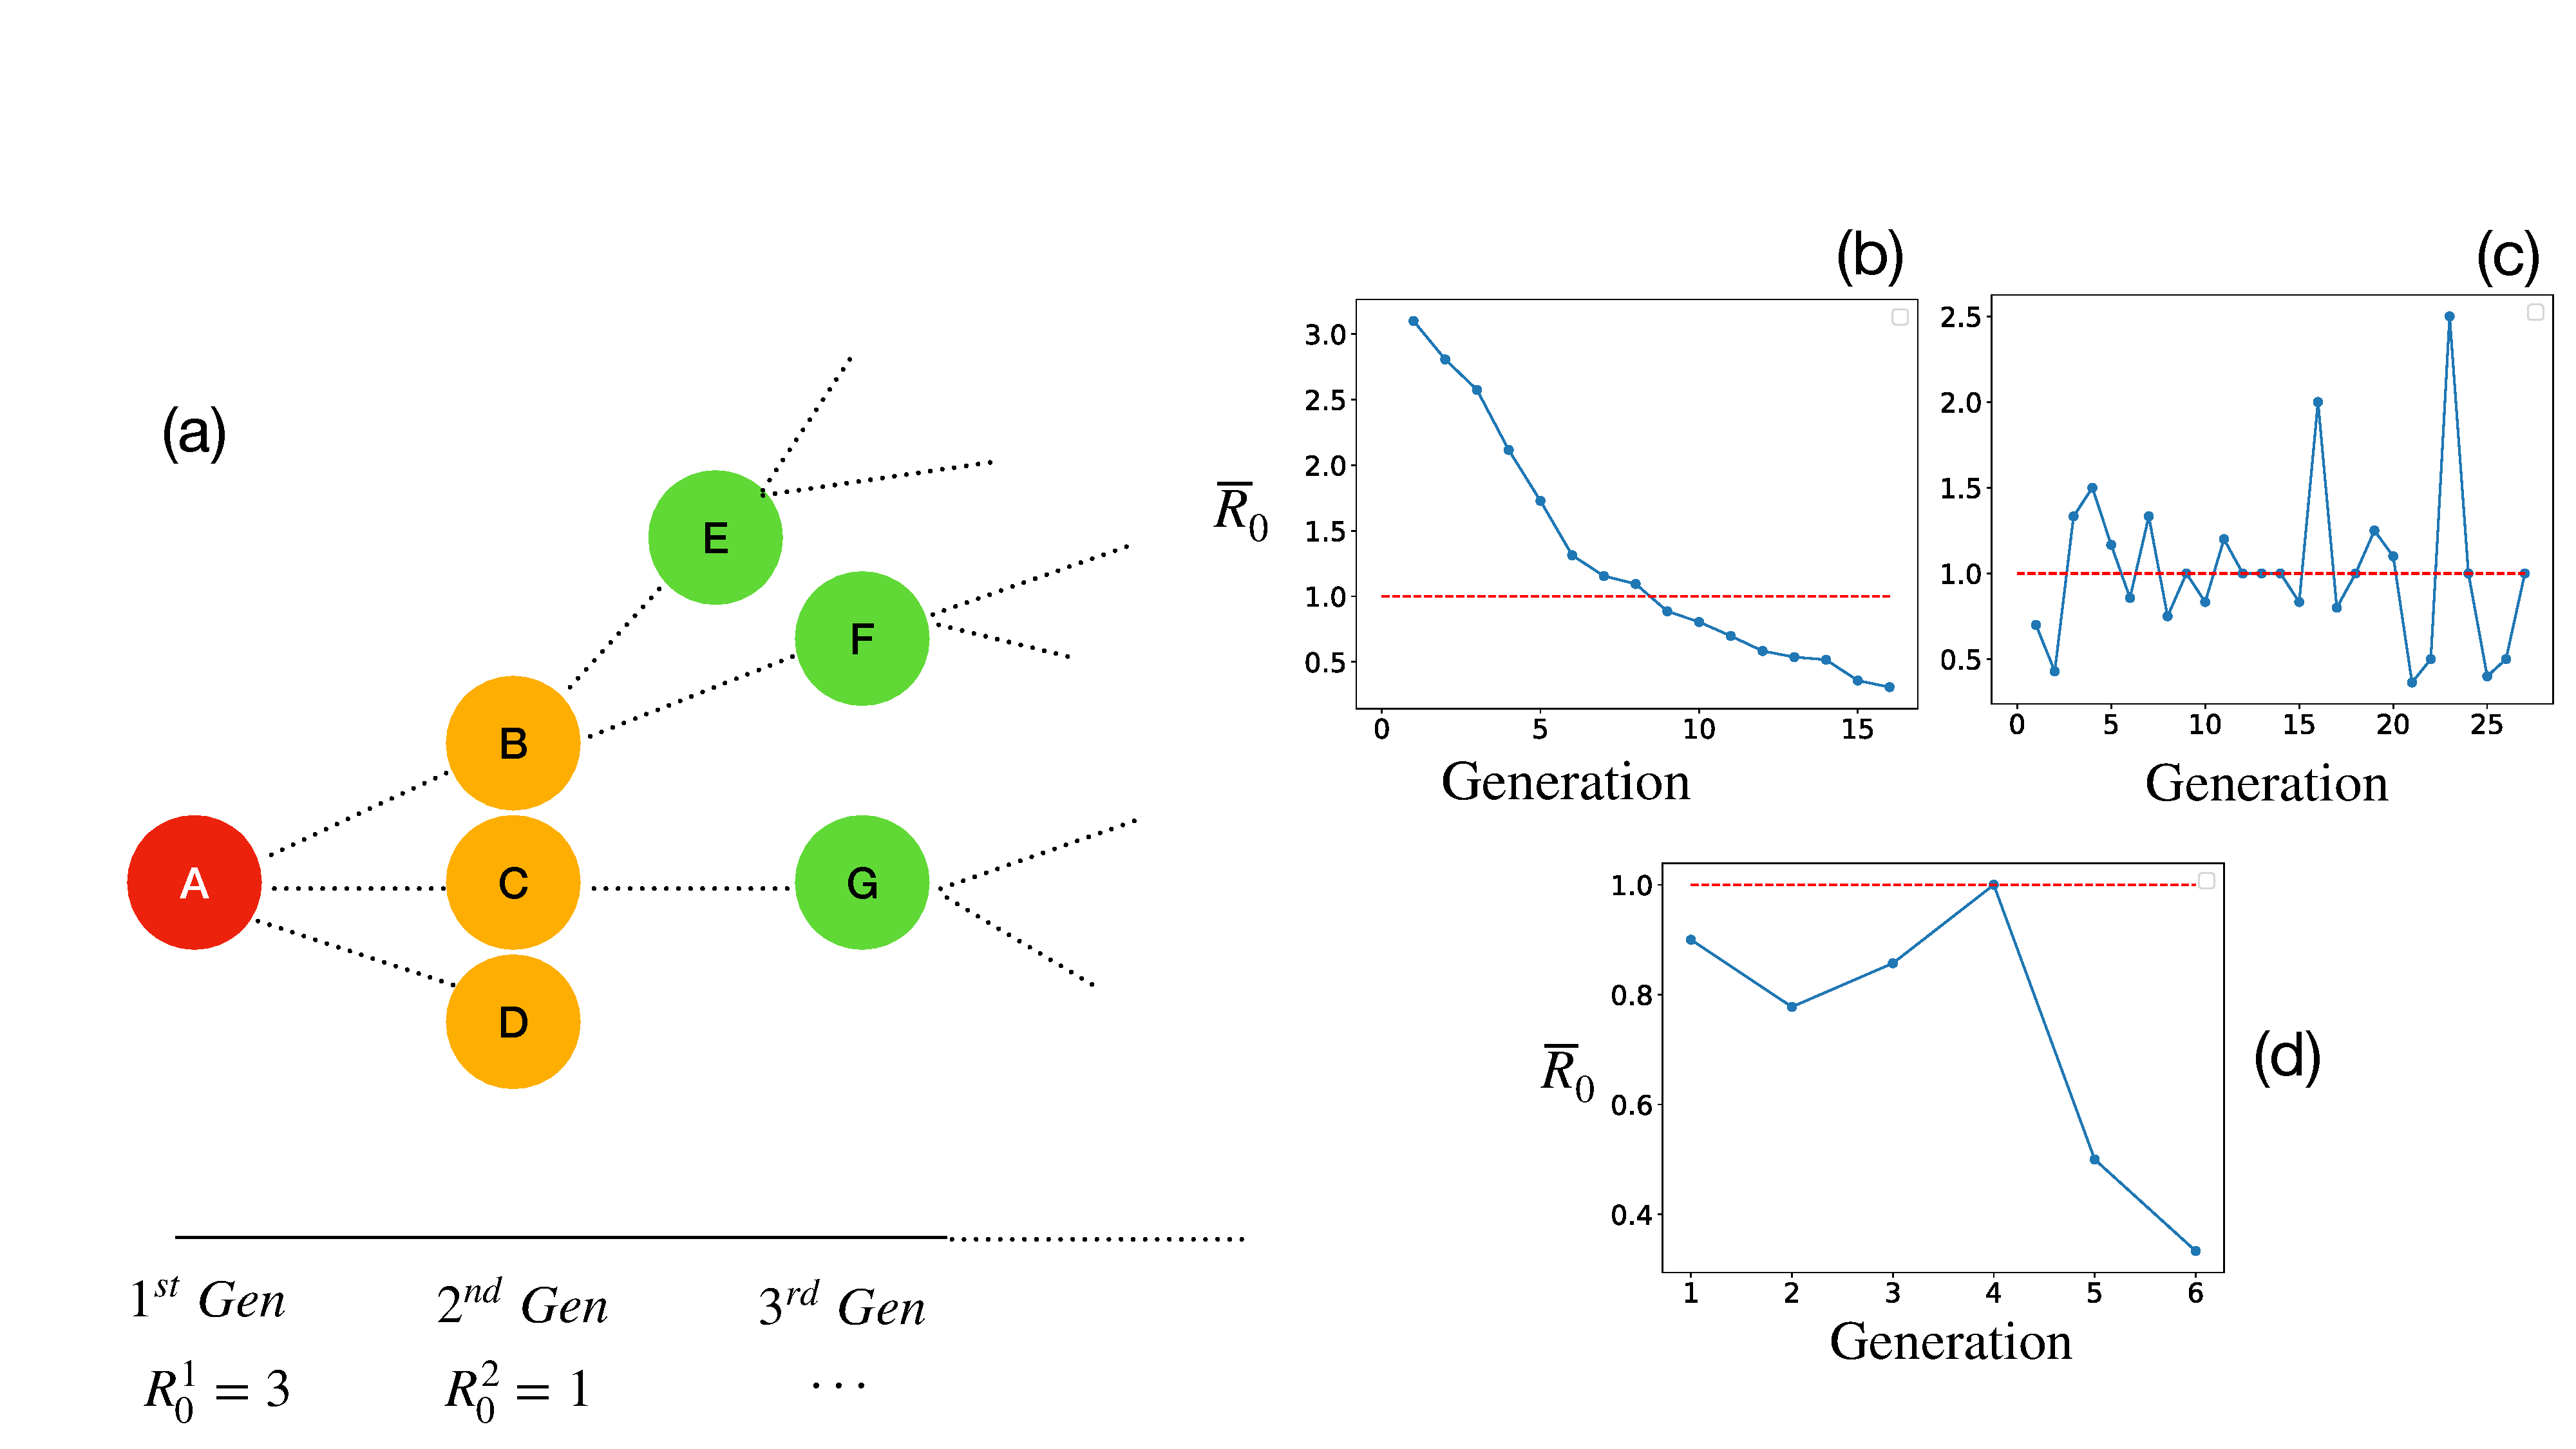
\includegraphics[scale=0.255]{chapter5/figures/fig1.pdf}
    \caption{Contact-traced $R_0$, the 'true' $R_0$. Tracking the history of all infected trees allows us to count how many infections are produced for each infectious tree over a simulation. At $t=0$, a single ($1^{st}$-generation) infection is positioned at the center of the domain. The quantity $R^i_0$ is defined as the mean number of infections produced for  the $i^{th}$ generation.}
    \label{fig:contact-trace}
\end{figure}

\subsection{Capturing $R_0$ in space and time}

For high levels of infection, the number of secondary infections are reduced because a lower number of susceptible trees are available to infect. 

In Figure \ref{fig:contact-trace}(b), we can see that measuring $R_0$ in a typical simulation, %
will likely over-estimate the contagiousness of the pathosystem at earlier times. %
Whereas, if $R_0$ is measured for later times (and the pathogen is above threshold), an %
under-estimate of the pathosystem contagiousness is likely. %
This is intuitive because the density of susceptible neighbors is higher at earlier times, %
on account of the neighborhood being untouched by other infected trees. %
The converse is true for later times in the simulation producing under-estimates. %
The number of secondary-infected trees will thus vary over time\footnote{Variations can %
also be expected at different locations through the domain. That is, centrally-distributed %
trees would, in theory, have access to infected more susceptible neighboring than trees %
located on the edge of the domain.}. %

Figure \ref{fig:contact-trace}(c) reveals how the pathosystem can behave if the threshold for %
invasion is just satisfied. %
Here $R_0$ is just above threshold for earlier times and barely spreads, however, the spread is chaotic. %
This can be considered a non-local generalisation of the SLM spreading on the critical point. %
In this scenario, $R_0$ is not strongly dependant on time. %
In the below-threshold regime, $R_0$ remains below $1$ for all generations and dies out after %
two generations. %

From Figures \ref{fig:contact-trace}(b-d), we have demonstrated that this definition of $R_0$ %
reliably captures the threshold of transmission during the initial stage of infection. %
Undesirably, we have made simplification in the assumptions and have not achieved a complete %
characterisation of $R_0$\textemdash which could, in be defined in terms of a growth %
rate per generation \cite{R0-construct}. %

We have not considered the re-growth of susceptible trees. %
If the number of susceptible hosts is fixed, without replacement, the number of susceptible hosts %
will continually decrease in time if an epidemic takes hold. %
This will reduce $R_0$ drastically for later time-periods. %
It appears inescapable that tree and plant-based systems violate the well-mixed population %
assumption that classic definitions of $R_0$ are based on. %
\textcolor{red}{Investigate how the next generation operator is used in the literature.}\\

% Averaging R0 over the entire ensemble will reduce R0, thus flatten the R0 map and reduce the amount of spatial clustering we see -- could illustrate this with a figure.

\subsection{$R_0$ and spatial scale}

Given that we have now defined $R_0$, we will investigate how this quantity changes in relation %
to the parameters dictating the spatial scale in our model. %
The parameters of interest are domain size $L$ and scale parameter $\alpha$. %
The domain size $L$ controls the array dimension stored in  memory, while $\alpha$ %
describes the physical space per-point inside the array i.e. the model resolution. %
The number of infections produced for each generation, $R_0^i$, were ensemble averaged with %
different values of domain size $L$ and scale parameter $\alpha$, %
shown in Figure \ref{fig:R0-spatial-scale}. Simulations started with a single infected, %
primary source, tree at the center of the domain and continued until the primary source %
transitioned into $I\rightarrow R$. %
The final number of contact-traced secondary infections produced from the primary infection %
constitute $R_0$.\\

The scale parameter of $5\mathrm{m}$, together with $L$, describe a range of different modelled %
areas which could represent fields, forests, stands or patches of land etc\footnote{Throughout this chapter, %
we take the domain to represent the average density of trees through a landscape.}. %
In Figure \ref{fig:R0-spatial-scale}(a), we can see values of $R_0^i$ increase with $L$ and %
begin to saturate to constant levels with a domain size $L\times L=1000\times 1000$, or $5\mathrm{km}\times 5 \mathrm{km}$. %
Beyond which, changes in domain size had negligible effects on $R_0$. %
This suggests for domain-sizes, up to some limit, the invasiveness of the pathogen has a %
dependence on the domain-size within which we choose to measure the spread. %
The result of Figure \ref{fig:R0-spatial-scale}(a) falls nicely in line with the work of %
others \cite{mikaberidze2016invasiveness} and suggests that the spatial scale is likely to %
alter the threshold of invasion.\\

The result of Figure \ref{fig:R0-spatial-scale}(a) is intuitive. %
Suppose we decide to calculate $R_0$ for a \textit{small} patch of land at density $\rho$, %
given a number of infected trees. In the case of wind-dispersal, it is clear to see that some %
innoculum (e.g. spores) would disperse out of the patch of land and infect other trees in %
neighbouring patches we are not considering. The value of $R_0$ is therefore subject to %
under-estimation for domain sizes small in comparison to the scale of dispersal.\\ 

On the other hand, suppose we measure $R_0$ for a larger patch of land at the same density $\rho$. Here, it is clear to see that we would count more secondary infections per infected tree and therefore measure a higher value of $R_0$. That is, the majority of dispersed inoculum will now land inside the domain boundary and directly effect the trees we are considering. At some point increasing the domain size will have no effect on $R_0$. This is likely to occur when the amount of inoculum, produced per tree\footnote{In our case $\beta$ represents a simplified compound parameter incorporating the amount of spores produced per tree and the probability of spore uptake by another $S$-tree.}, saturates the domain with only negligible amount of dispersing out of the patch.\\

\begin{figure}
    \centering
    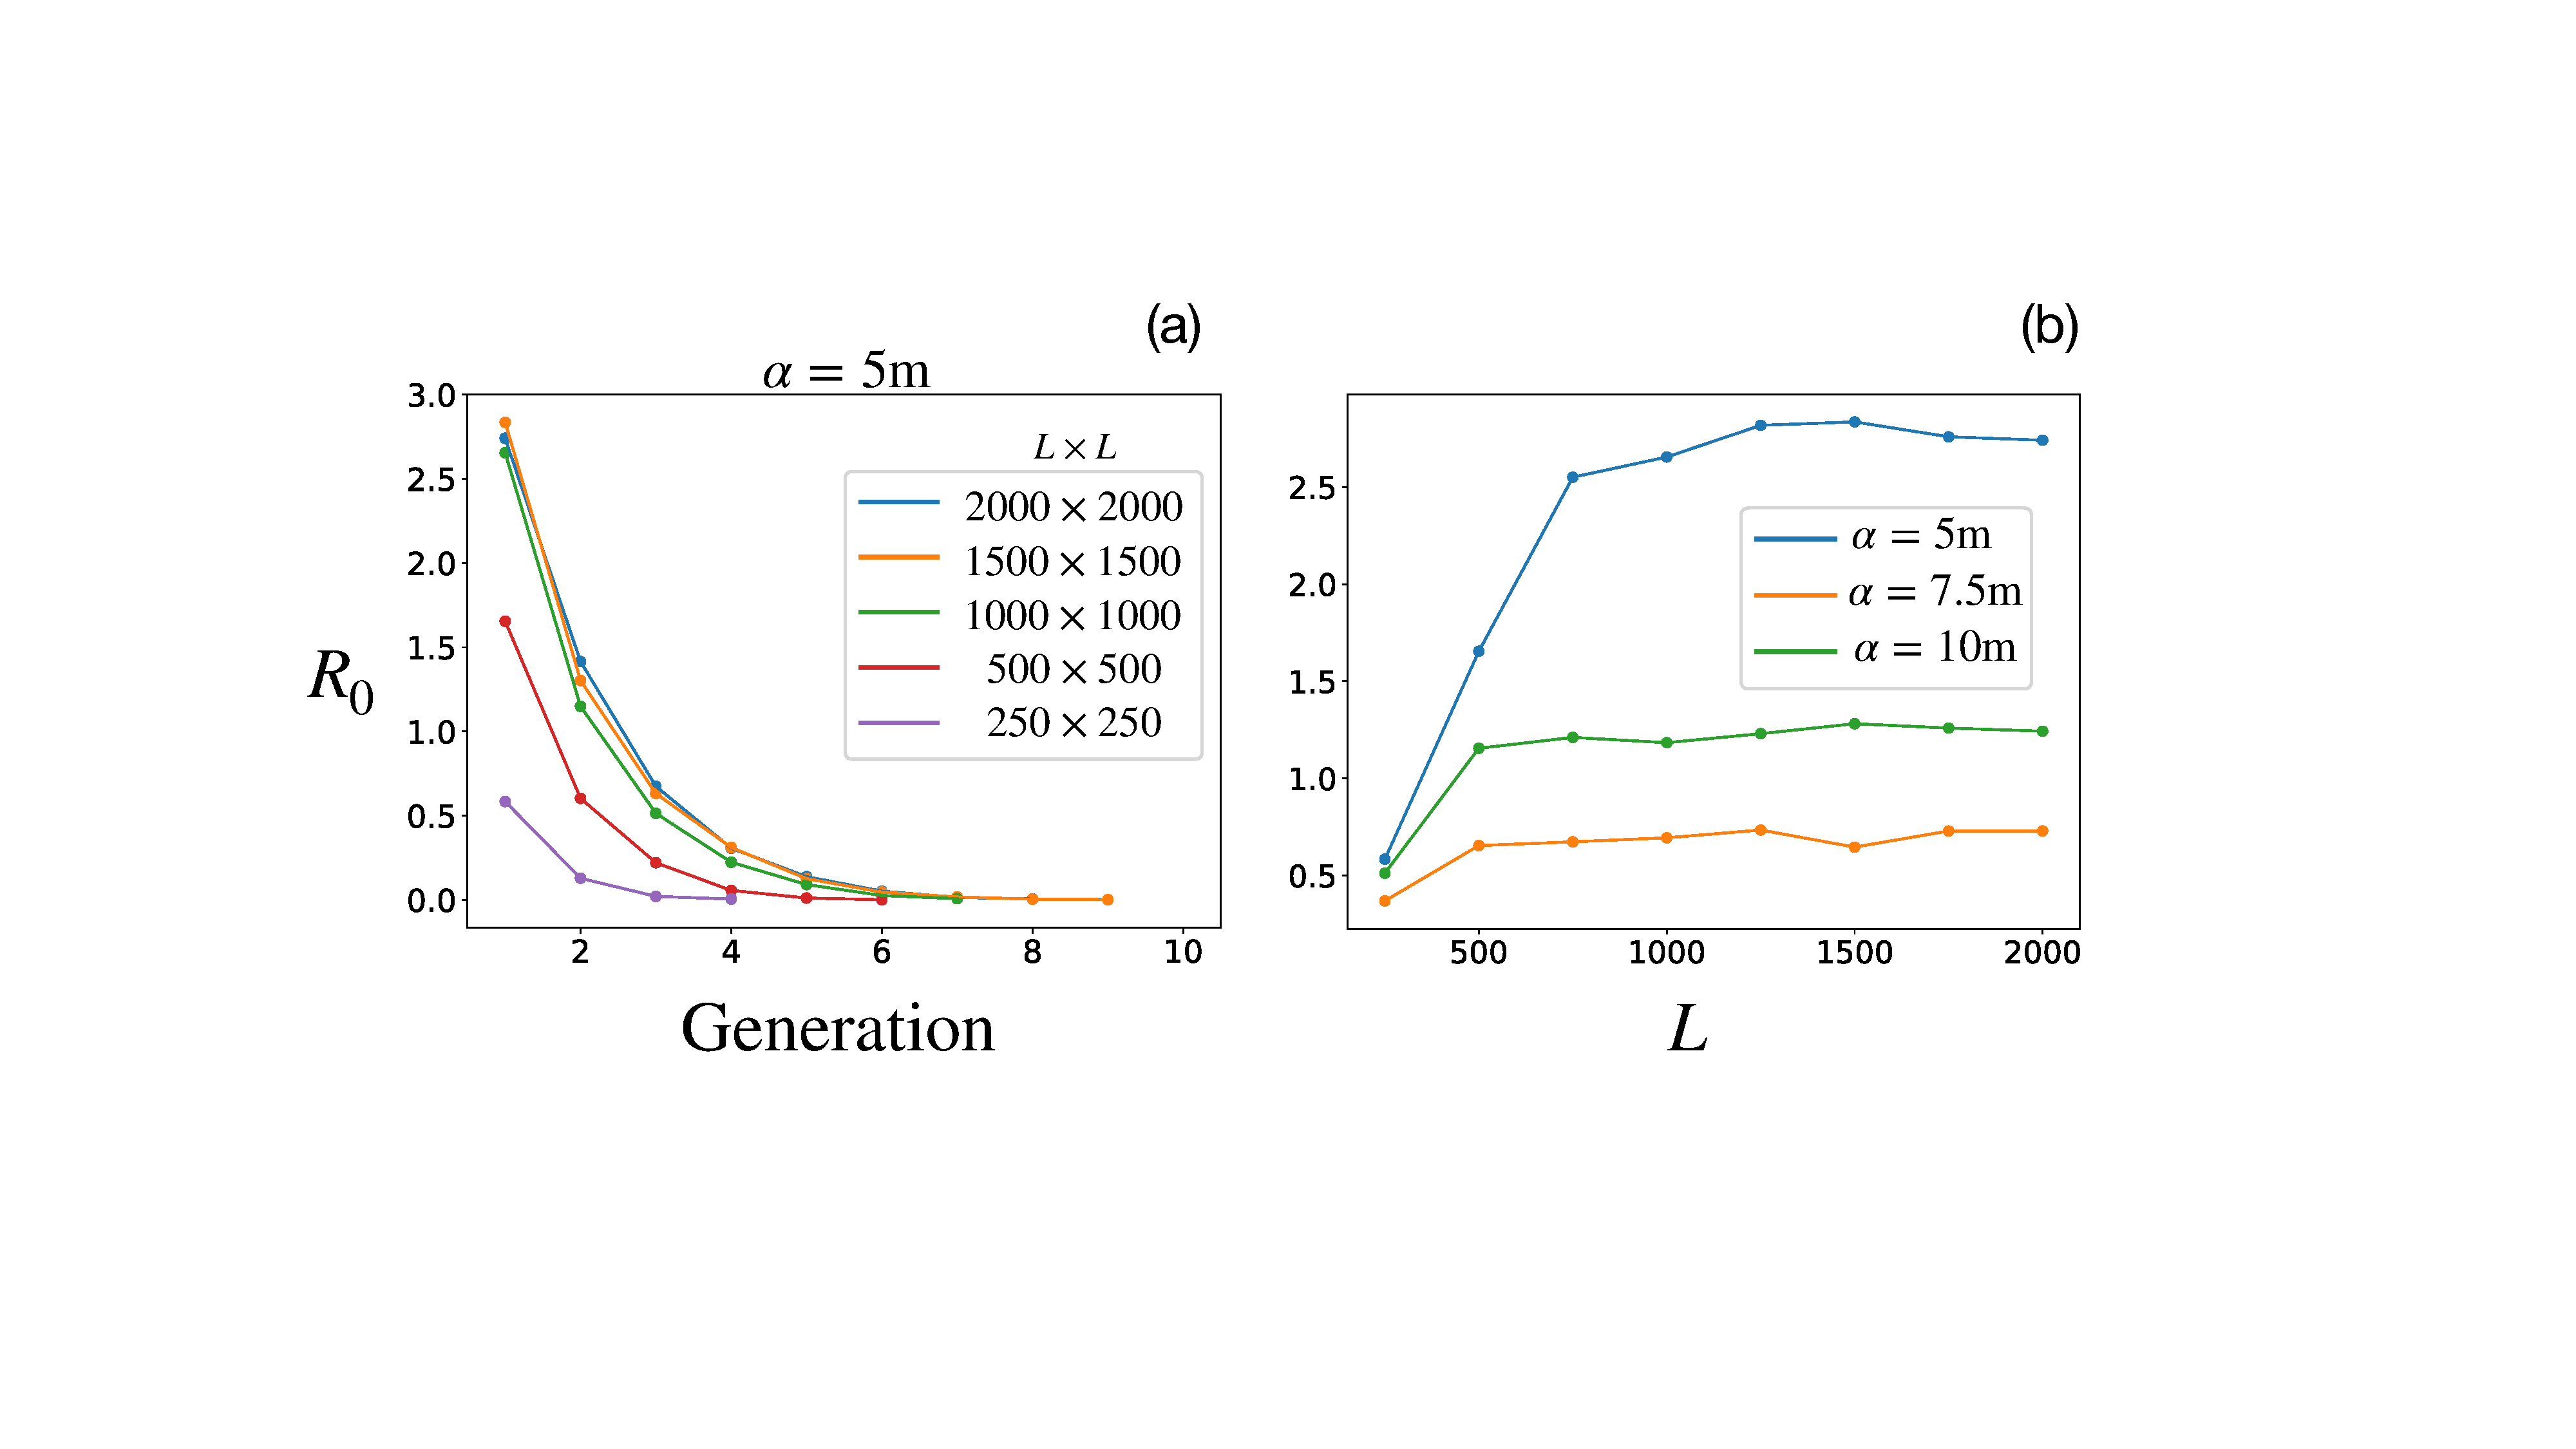
\includegraphics[scale=0.3]{chapter5/figures/fig2.pdf}
    \caption{How $R_0$ depends on scale...}
    \label{fig:R0-spatial-scale}
\end{figure}

Figure \ref{fig:R0-spatial-scale}(b) shows the model behaviour when the scale parameter is %
changed in conjunction with the domain size $L$. From this we notice a drastic and surprising %
reduction in the scale of pathogen spread for higher $\alpha$. %
This points towards a limitation in our model infectivity parameter $\beta$. %
Increasing $\alpha$ has the effect of increasing the average spacing between trees and %
increasing effective host canopy cover. %
In changing $\alpha$, the spatial resolution is rescaled and the expectation is that a higher value of $\beta$ should be seen to reflected a larger canopy cover. %
The infectivity $\beta$ represents a simplified compound parameter that incorporates information about the spore production rate. %
Re-scaling the canopy cover means more susceptible plant material can become infected and produce further spores. 
% JS_what does this mean 
\textcolor{red}{Tighten me up, talk about me to group.}\\

% beta is a per-capita rate of infection, that can be seen as a compound parameter...


\section{Inverse power law dispersal}

% - explore the scale parameter and the exponent 
% - show that for the same value of R0 exponent and scale parameter combinations yield a faster spread

\blindtext 

\blindtext


\section{Invasiveness: patch-to-patch transitions}

\blindtext

\blindtext

\blindtext

\section{Chapter summary}

\blindtext

\blindtext
